\begin{enumerate}[label=\thechapter.\arabic*,ref=\thechapter.\theenumi]
\item
For the circuit given below, choose the angular frequency $ \omega_0$ at which voltage across capacitor has maximum amplitude?
\begin{figure}[h!]
    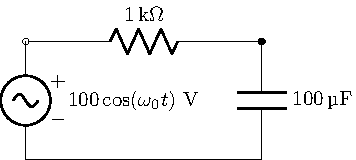
\includegraphics[width = 0.5\columnwidth]{2023/BM/16/figs/c_fig1.pdf}
    \caption{circuit }
    \centering
    \label{fig: bm_16_fig_1}
\end{figure}
\begin{enumerate}
    \item[(A)] 1000
    \item[(B)] 100
    \item[(C)] 1
    \item[(D)] 0   
\end{enumerate}
\hfill(GATE BM 2023 Question 16)\\

\item 
A finite impulse response (FIR) filter has only two non-zero samples in its impulse response $h[n]$, namely $h[0] = h[1] = 1$. The Discrete Time Fourier Transform (DTFT) of $h[n]$ equals $H(e^{j\omega})$, as a function of the normalized angular frequency $\omega$. For the range $\abs{\omega} \leq \pi$, $\abs{H(e^{j\omega})}$ is equal to
\begin{enumerate}
	\item[(A)] $2\abs{\cos(\omega)}$
	\item[(B)] $2\abs{\sin(\omega)}$
	\item[(C)] $2\abs{\cos(\frac{\omega}{2})}$
	\item[(D)] $2\abs{\sin(\frac{\omega}{2})}$
\end{enumerate}
\hfill(GATE BM 2023 Question 17) \\
\end{enumerate}
